\chapter{Detection of bank lines} \label{Chp3}

The location of bank lines is determined by looking at the transition of water to land at a reference discharge computed with a D-Flow FM model.
To determine the exact location of the bank lines, first all cells in the D-Flow FM-grid are marked that are at the transition from land to water at these discharge level.
The concerned cells have positive water depth and one or more neighbouring cells with a zero water depth.
Within these transition cells a bank line can be defined.
The bank line is at the location where the water depth is equal to zero, that is the water level is equal to the bed level.
In D-Flow FM the bed level, $d$ , is defined in the corner points of a cell and the water level, $z$ , in the centre of a cell, see \autoref{Fig3.1}.
The bank line is now found by interpolating the bed level linearly along the grid lines and marking the location where the bed level is equal to the water level.
In this way, two points are found which can be connected to form (a part of) the bank line.

\begin{figure}
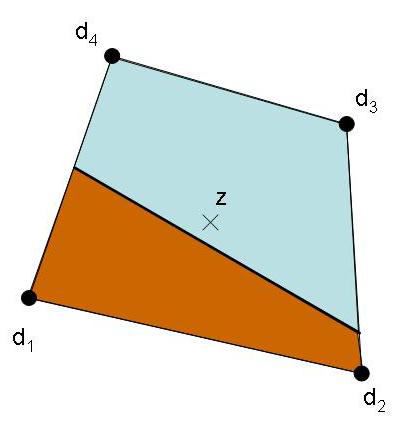
\includegraphics[width=5cm]{figures/Fig3-1.png}
\caption{Location of a bank line within a transition cell}
\label{Fig3.1}
\end{figure}

An example is given in \autoref{Fig3.1}, where $d_1$ and $d_2$ are smaller than $-z$ en $d_3$ en $d_4$ larger than $-z$ (water depth $h = z+d$ ).

The found locations of the bank lines will depend on the chosen discharge level.
However, as long as the discharge is within the main channel, the locations will be fairly constant.

Generally, bank erosion only within the main channel.
It is therefore possible to only take into account those cells that are within a certain range of predefined lines.
This is also necessary when more than one bank line is present (as is common in rivers), because otherwise it is not clear which coordinates belong to one bank or the other.

For the Dutch rivers 'oeverlijnen' from Baseline can be used for these pre-defined lines.
These lines should be defined in a simple text file consisting of x- and y- coordinates (\command{Line1}, ..., \command{LineN}, in the definition file).

One of the disadvantages of the 'oeverlijnen' from Baseline is that they only depict the main channel.
Possible side channels, shortcuts or lakes will then not be detected by the tool, see \autoref{Fig3.2}.
If they are important, extra lines should be added that (globally) represent the bank lines of these features.

\begin{figure}
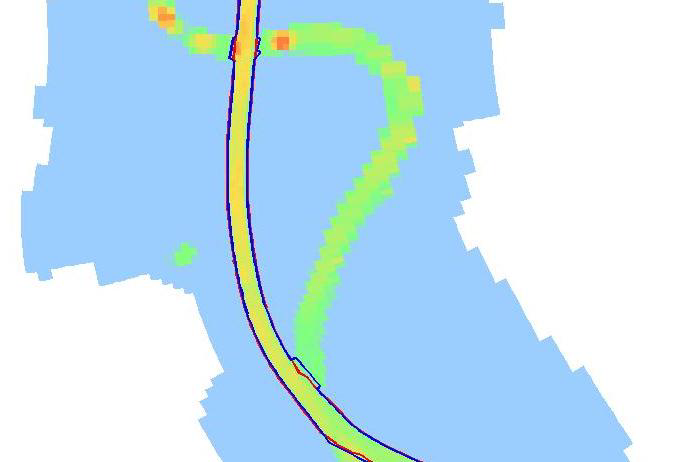
\includegraphics[width=\textwidth]{figures/Fig3-2.png}
\caption{Detection of bank lines at a shortcut in the Muese river.
Red: Baseline 'oeverlijnen', Blue: detected bank line from D-Flow FM computation (Q = 278.5 m\textsuperscript{3}/s, average discharge)}
\label{Fig3.2}
\end{figure}

Groynes are not detected as such by the tool, because they are defined on subgrid level in D-Flow FM, see \autoref{Fig3.3}.
The detected bank line is in this case following the banks within groyne sections.
This is an advantage, since possible bank erosion only takes place in the groyne sections and not along the groynes themselves.

\begin{figure}
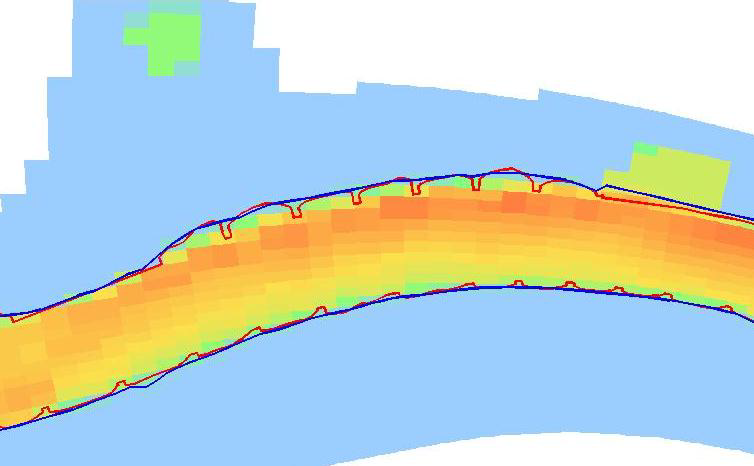
\includegraphics[width=\textwidth]{figures/Fig3-3.png}
\caption{Detection of a bank line close to groynes.
Red: Baseline 'oeverlijnen', Blue: detected bank line from D-Flow FM computation (Q=278,5 m\textsuperscript{3}/s, average discharge)}
\label{Fig3.3}
\end{figure}